\documentclass{standalone}

\usepackage{tikz}

\def \D { 
    (0,0) , (3,0) , (6,0) , (9,0) , (12,0) , (15,0)  , 
    (2,1) , (5,1) , (8,1)  ,  
    (1,2) , (4,2) , (13,2) , (16,2)  , 
    (9,3) , (12,3) , (15,3)  , 
    (2,4) , (11,4)  , 
    (10,5) , (16,5)  , 
    (3,6) , (9,6)  , 
    (2,7) , (8,7) , (17,7)  , 
    (1,8) , (16,8)  , 
    (0,9) , (9,9) , (15,9)  , 
    (8,10) , (14,10)  , 
    (1,11) , (7,11)  , 
    (6,12) , (15,12)  , 
    (2,13) , (5,13) , (8,13)  , 
    (1,14) , (4,14) , (13,14) , (16,14)  , 
    (9,15) , (12,15) , (15,15)  , 
    (2,16) , (5,16) , (8,16) , (11,16) , (14,16) , (17,16) }

\def \A { 
    (0,0) , (3,0) , (12,0) , (15,0) , 
    (8,1) ,  
    (1,2) , 
    (9,3) , (15,3) , 
    (2,4) , 
    (16,5) , 
    (8,7) , 
    (0,9) ,
    (14,10)  , 
    (1,11) , (7,11)  , 
    (15,12)  , 
    (8,13)  , 
    (1,14) , (4,14) , (13,14) , (16,14) }

\def \B { 
    (3,0) , (6,0) , (9,0) , 
    (2,1) , (5,1) ,  
    (13,2) , (16,2) , 
    (12,3) ,
    (11,4) , 
    (10,5) , 
    (3,6) , (9,6)  , 
    (2,7) , (17,7) , 
    (1,8) , (16,8) , 
    (9,9) , (15,9) , 
    (8,10) , 
    (7,11) , 
    (6,12) , 
    (2,13) , (5,13) , 
    (13,14) , (16,14) , 
    (9,15) , (12,15) , (15,15)}

\begin{document}
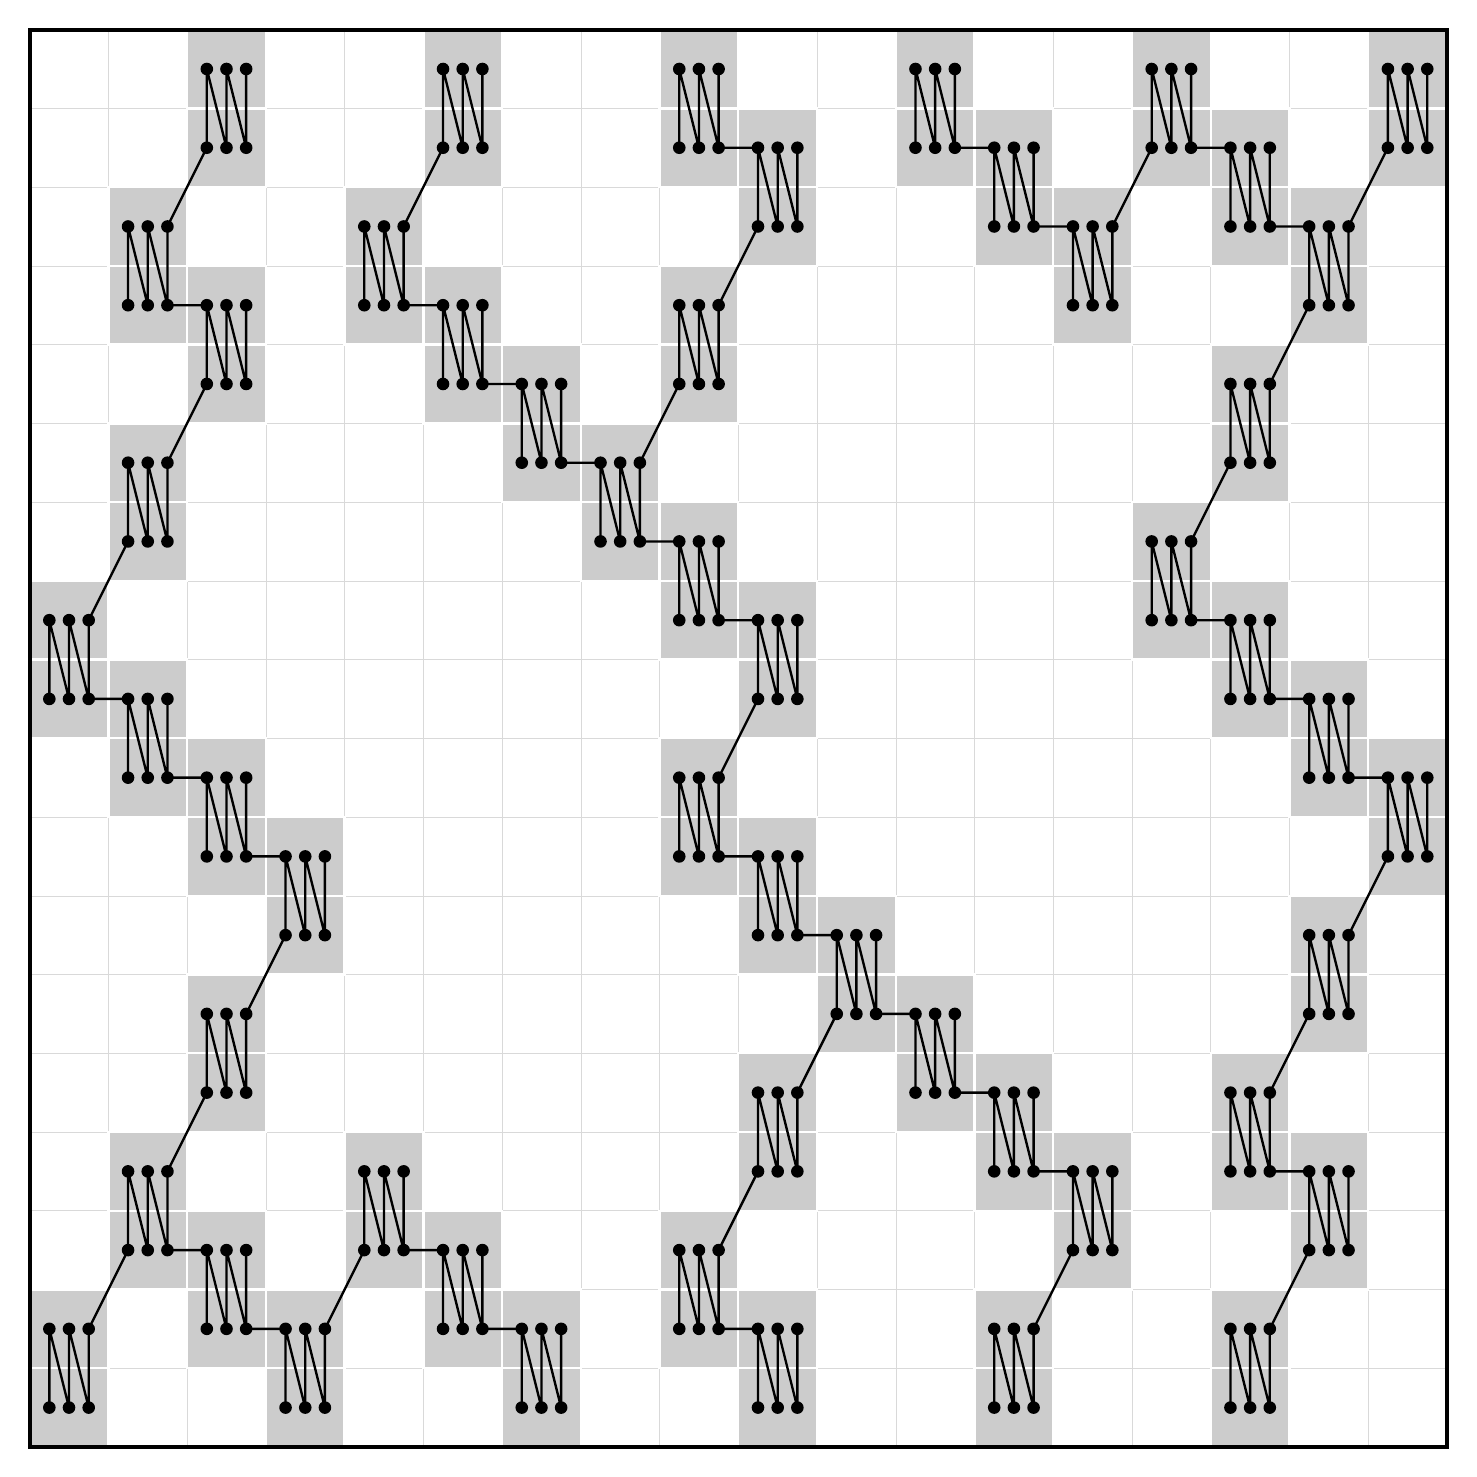
\begin{tikzpicture}
\draw[help lines, black!15] (0,0) grid (18,18);
\foreach \a in \D
    {\draw[black!0, fill=black!20, line width=0.3mm]
        \a rectangle +(1,1)
        \a++(0,1) rectangle +(1,1);
     \fill[black] foreach \b in 
        {(0.25, 0.5), (0.5, 0.5), (0.75, 0.5), (0.25, 1.5), (0.5, 1.5), (0.75, 1.5)}
        {\a++\b circle (0.8mm)};
     \draw[black, line width=0.3mm]
        \a++(0.25, 0.5)--+(0, 1)
        \a++(0.5, 0.5)--+(-0.25, 1)
        \a++(0.5, 0.5)--+(0, 1)
        \a++(0.75, 0.5)--+(-0.25, 1)
        \a++(0.75, 0.5)--+(0, 1);
    };
\draw[black, line width=0.3mm]
    foreach \a in \A
        {\a++(0.75, 1.5)--+(0.5, 1)}
    foreach \a in \B
        {\a++(0.25, 1.5)--+(-0.5, 0)};
\draw[black, line width=0.5mm] (0,0)rectangle (18,18);
\end{tikzpicture}
\end{document}